\documentclass[a4paper]{exam}

\usepackage{geometry}
\usepackage{graphicx}
\usepackage{hyperref}
\usepackage{titling}
% \usepackage[demo]{graphicx}
\usepackage{caption}
\usepackage{subcaption}
% \usepackage{subfigure}

\printanswers

\title{Assignment 1: Evolutionary Algorithm in action\\CS 451: Computational Intelligence}
\author{Ali Asghar Yousuf\\Muhammad Murtaza}  % <==== replace with your team name for grading
\date{Habib University | Spring 2023}

\runningheader{CS 451: Computational Intelligence}{Assignment 1: Evolutionary Algorithm}{\theauthor}
\runningheadrule
\runningfootrule
\runningfooter{}{Page \thepage\ of \numpages}{}

\qformat{{\large\bf \thequestion. \thequestiontitle}\hfill}
\boxedpoints

\begin{document}
\maketitle

\begin{questions}

  \titledquestion{Travelling Sales Person}
  The following are plots for respective selection schemes.

  \begin{figure}[!h]
    \centering
    \textbf{Fitness Proportional Scheme and Truncation}
    \begin{subfigure}{.5\textwidth}
      \centering
      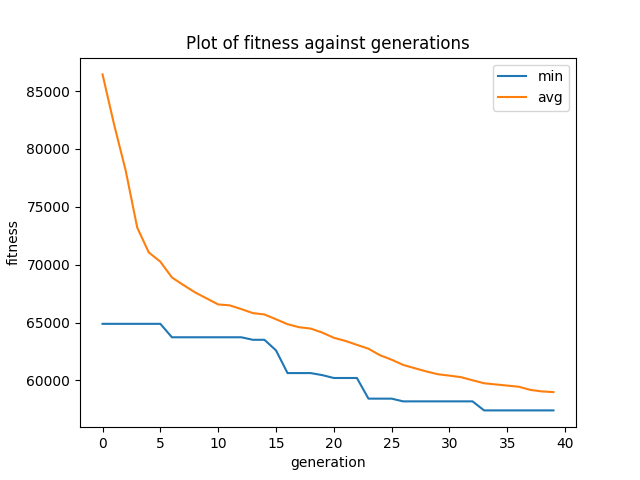
\includegraphics[width=1\linewidth]{tsp_min_avg}
      \caption{TSP Single run on 40 generations}
      \label{fig:sub1}
    \end{subfigure}%
    \begin{subfigure}{.5\textwidth}
      \centering
      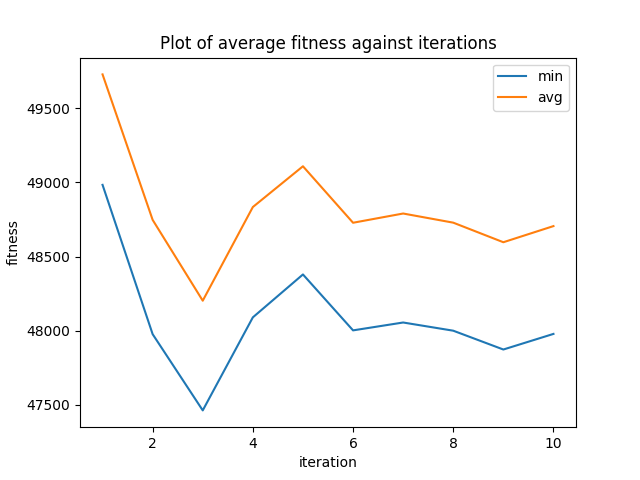
\includegraphics[width=1\linewidth]{tsp_itr_avg_2}
      \caption{TSP 10 runs on 1000 generations}
      \label{fig:sub2}
    \end{subfigure}
    \caption{Note: Fitness is the distance}
    \label{fig:test}
  \end{figure}
  % \begin{figure*}[!h]
  %   \centering
  %   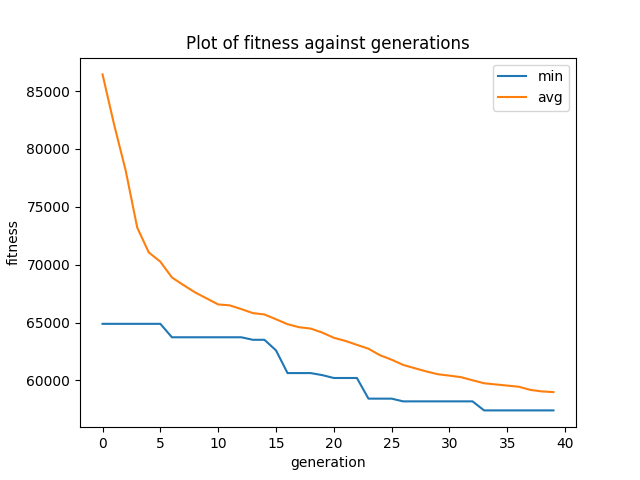
\includegraphics[width=.95\textwidth]{tsp_min_avg}

  %   \caption{TSP Single run on 40 generations\\Note: Fitness is the distance}
  %   \label{fig:notation}
  % \end{figure*}

\end{questions}

\end{document}